\chapter{Fluorescent neuronal cells dataset}
\label{chap:partI_dataset}

\begin{figure}
\centerline{
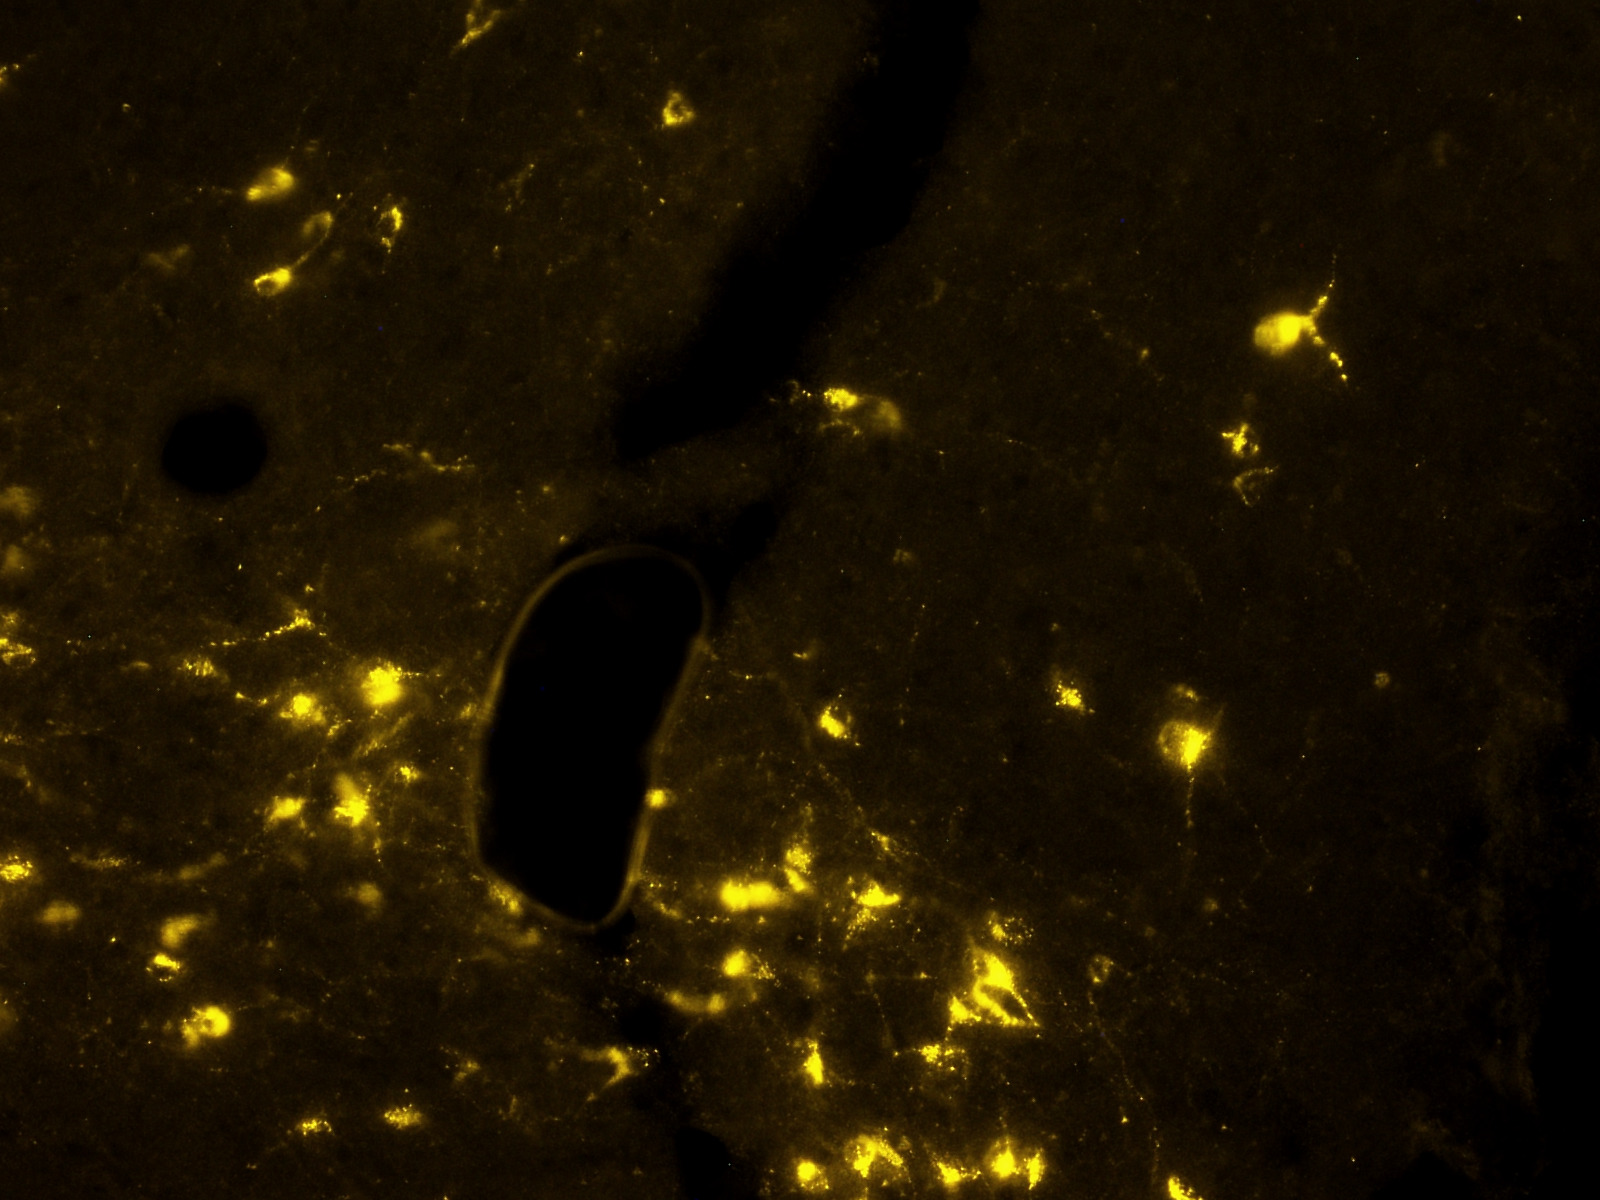
\includegraphics[width=0.55\textwidth]{figures/120_dataset/i_big_hole.jpeg}
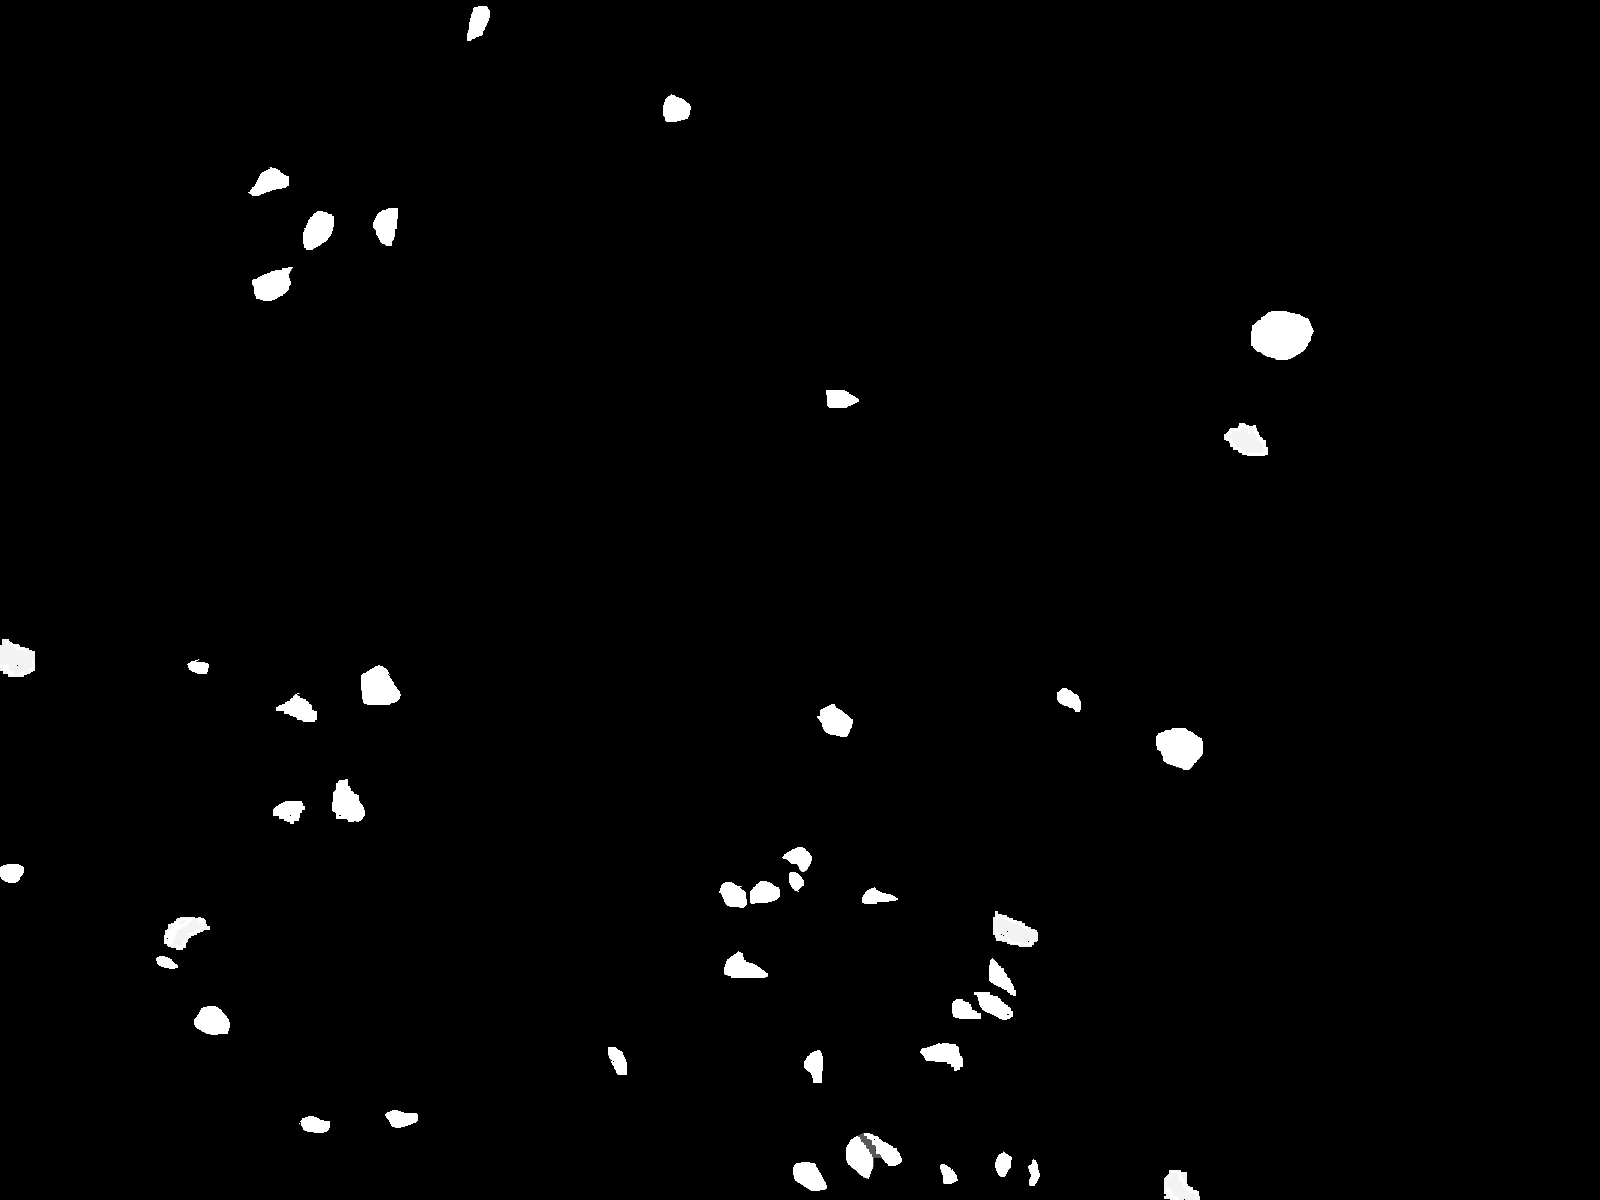
\includegraphics[width=0.55\textwidth]{figures/120_dataset/m_big_hole.png}
}
\centerline{
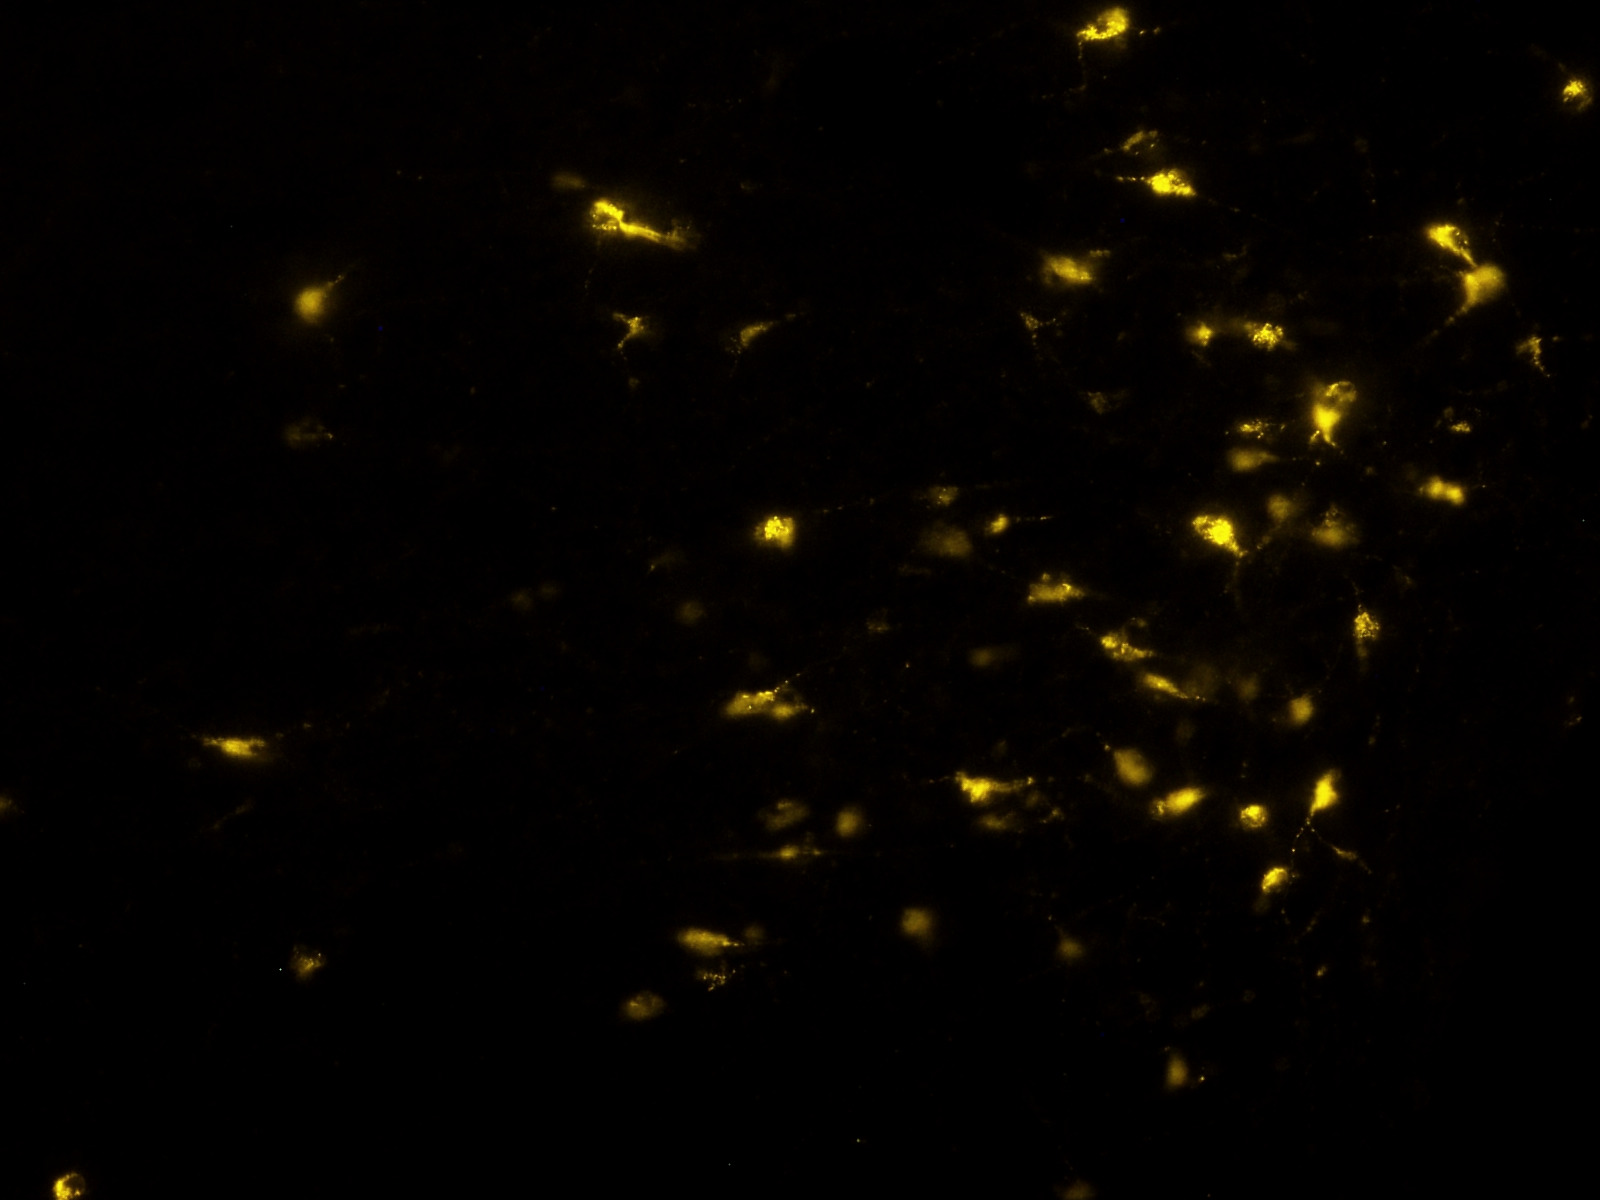
\includegraphics[width=0.55\textwidth]{figures/120_dataset/i_168.jpeg}
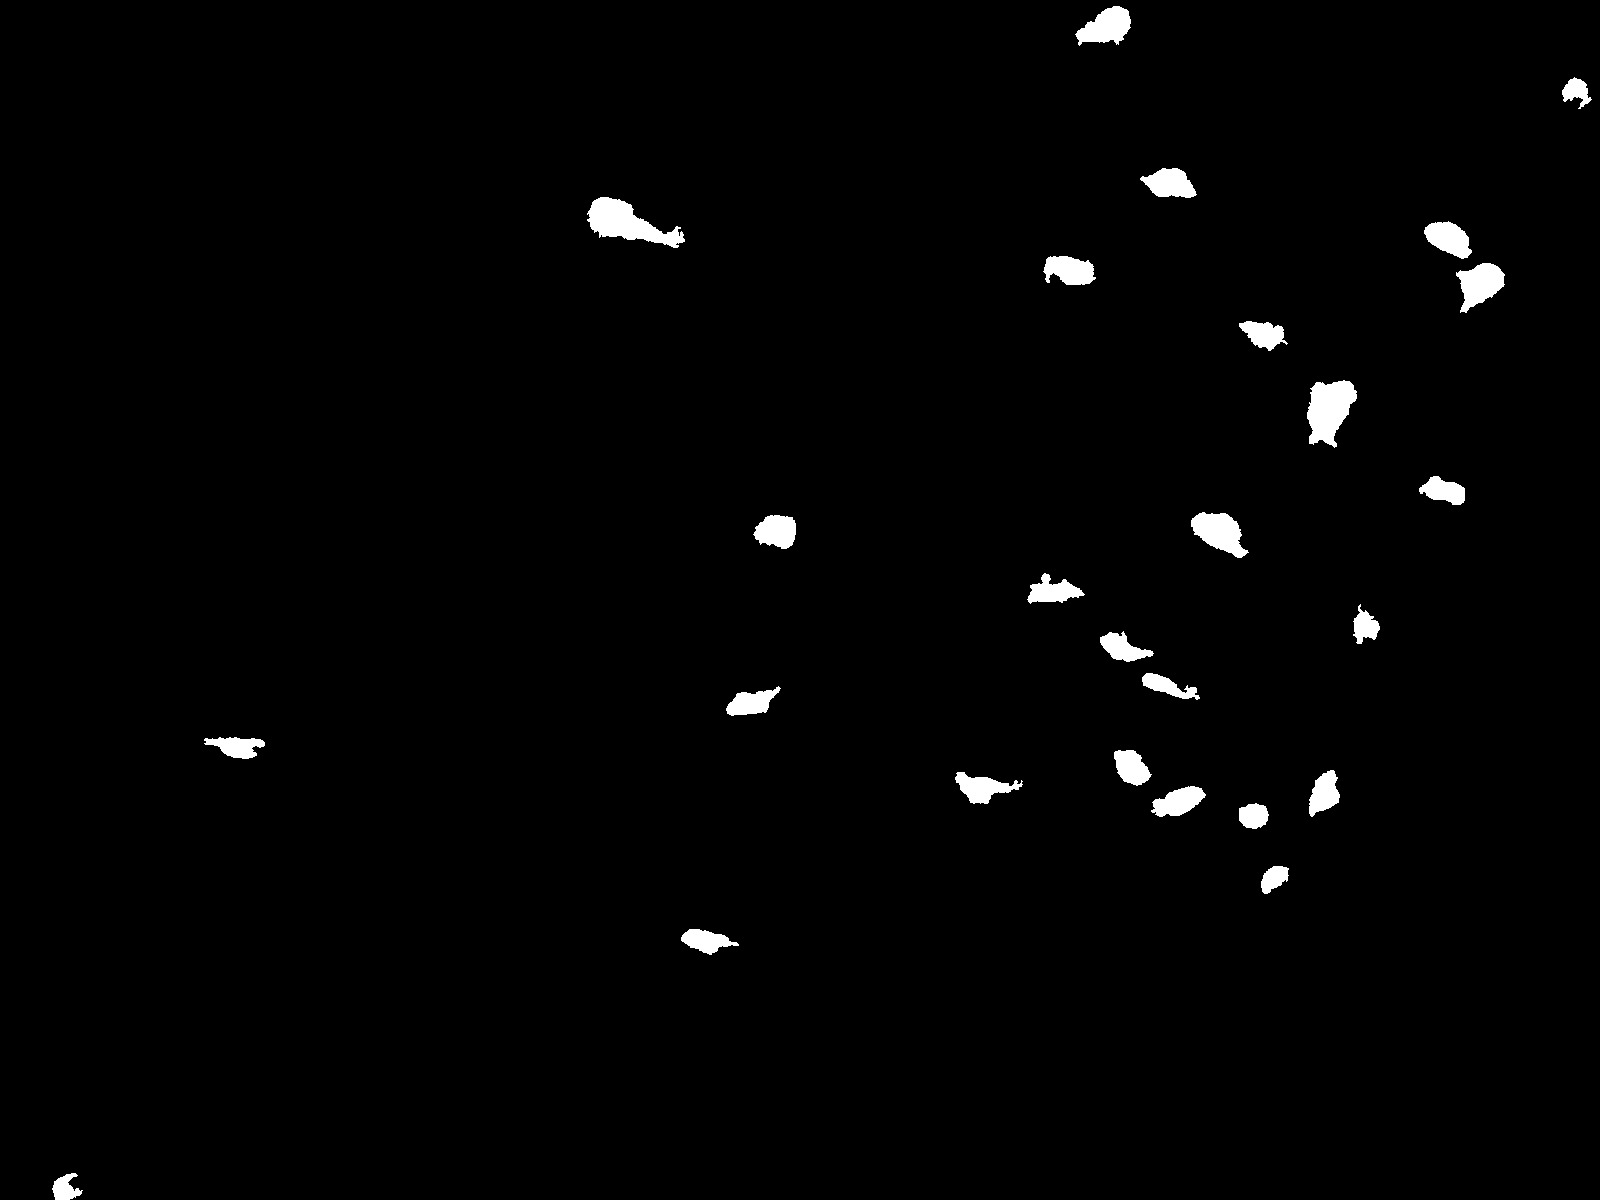
\includegraphics[width=0.55\textwidth]{figures/120_dataset/m_168.jpeg}
}
\centerline{
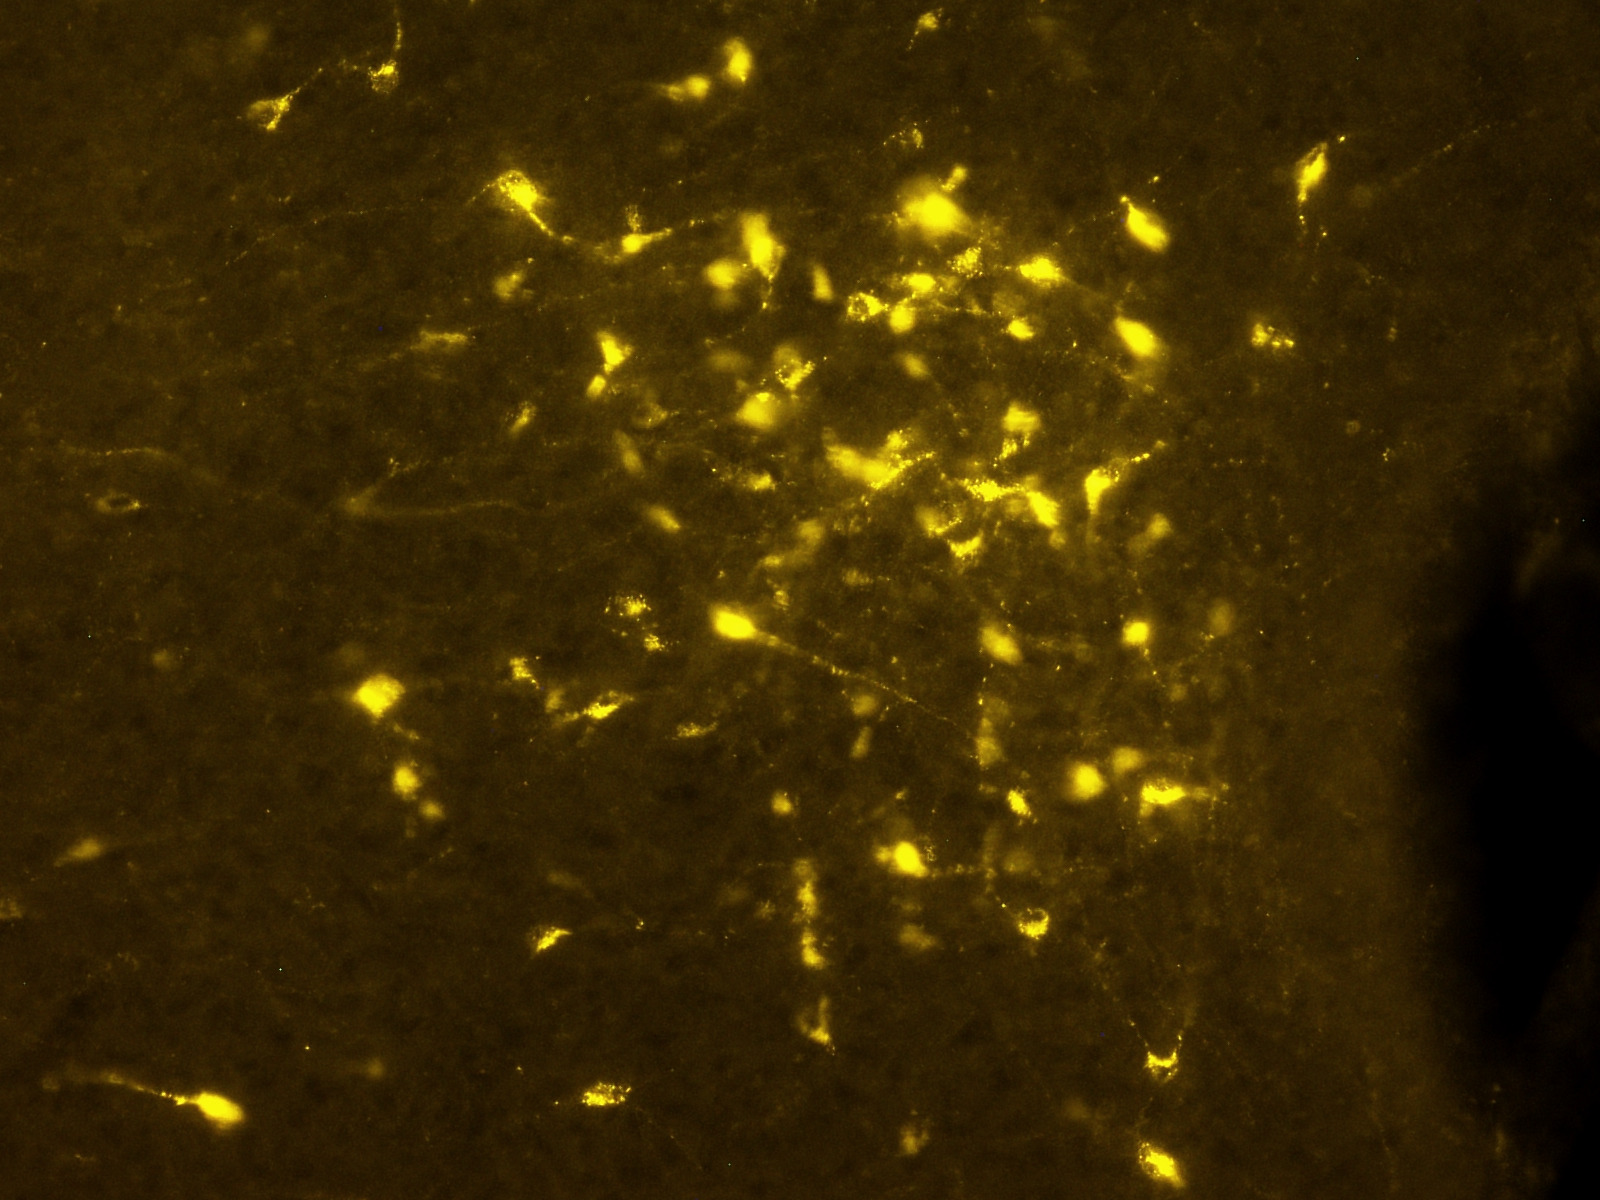
\includegraphics[width=0.55\textwidth]{figures/120_dataset/i_257.jpeg}
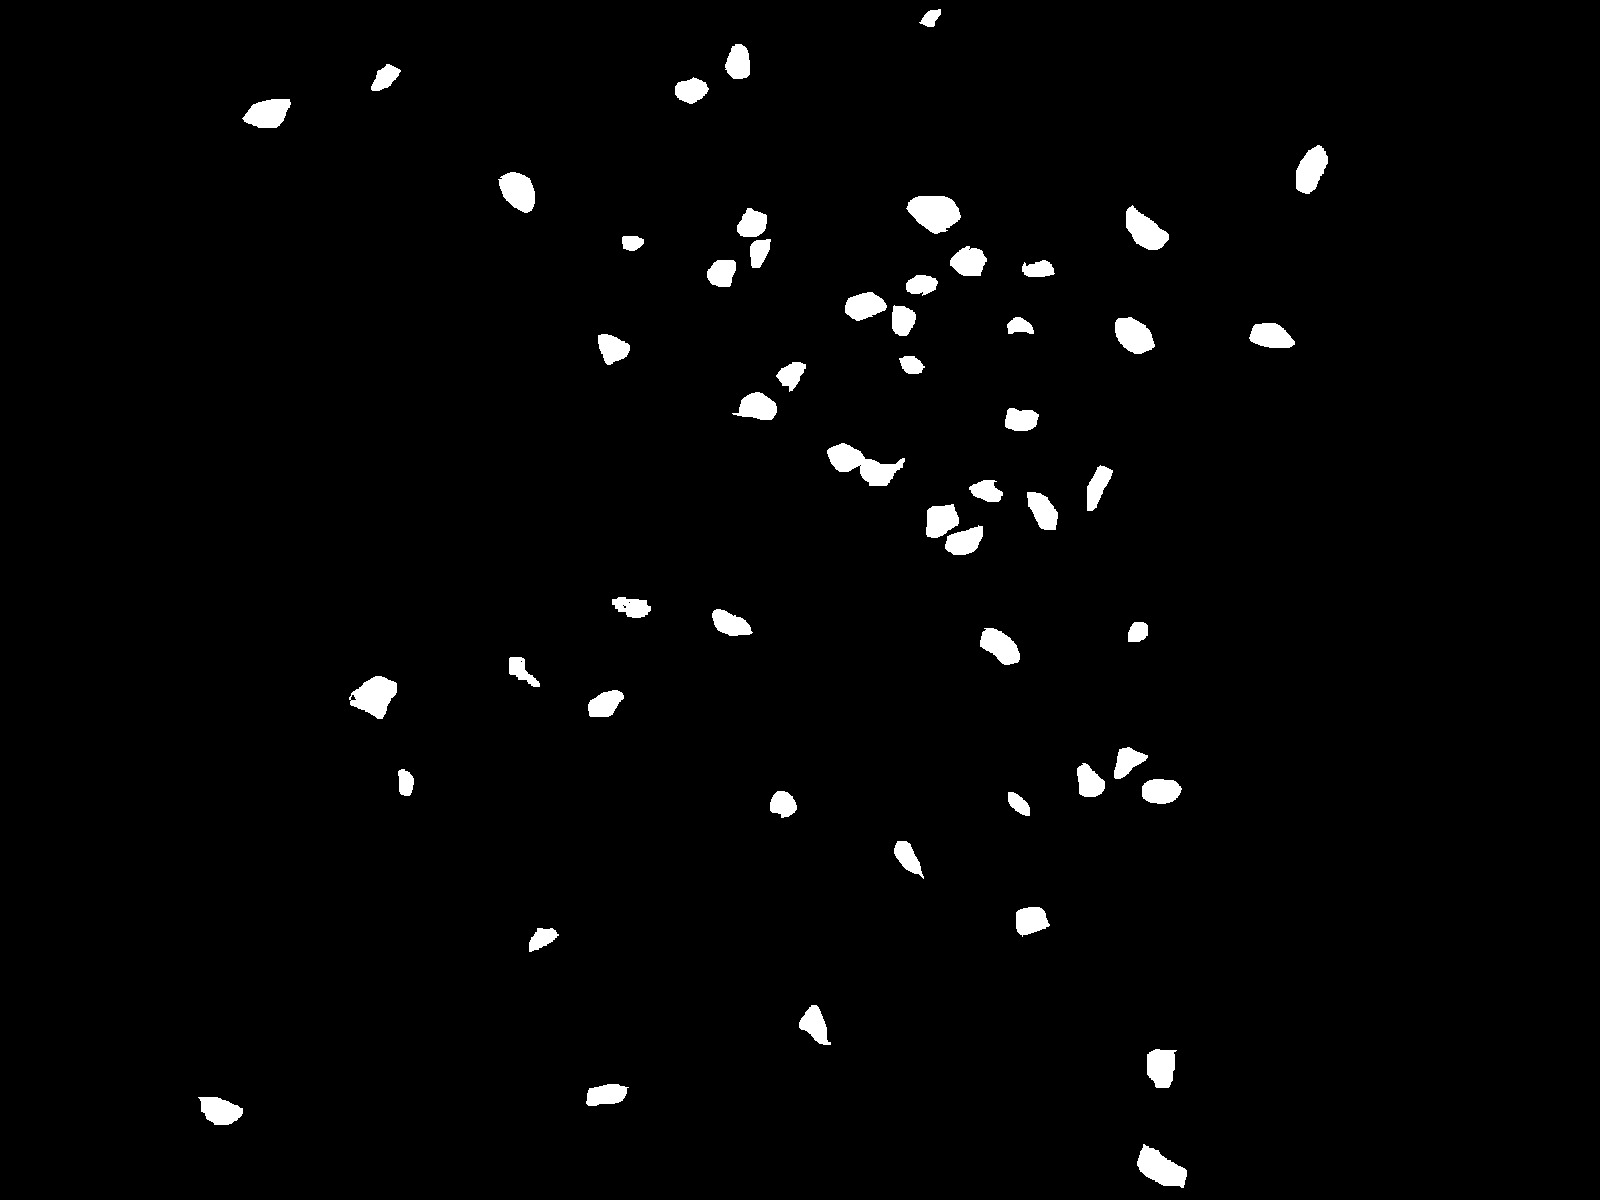
\includegraphics[width=0.55\textwidth]{figures/120_dataset/m_257.jpeg}
}
\label{fig:dataset}
\caption{
\textbf{Sample data}. The original images (left) present neuronal cells of different shape, size and saturation over a background of variable brightness and color.
The corresponding ground-truth masks used for training (right) depicts cells as white pixels over a black background.
%%rephrase
% \textbf{Sample data}. In the original images (left), the neuronal cells of interest appear as yellow spots over a background of variable brightness and color. They exhibit a large variability in terms of shape, size and saturation, which makes them hard to distinguish from artifacts and similar biological structures that are not of interest.
% The corresponding ground-truth masks used for training (right) depicts cells as white pixels over a black background.
} \end{figure}%
\begin{figure}[ht]\ContinuedFloat
\centerline{
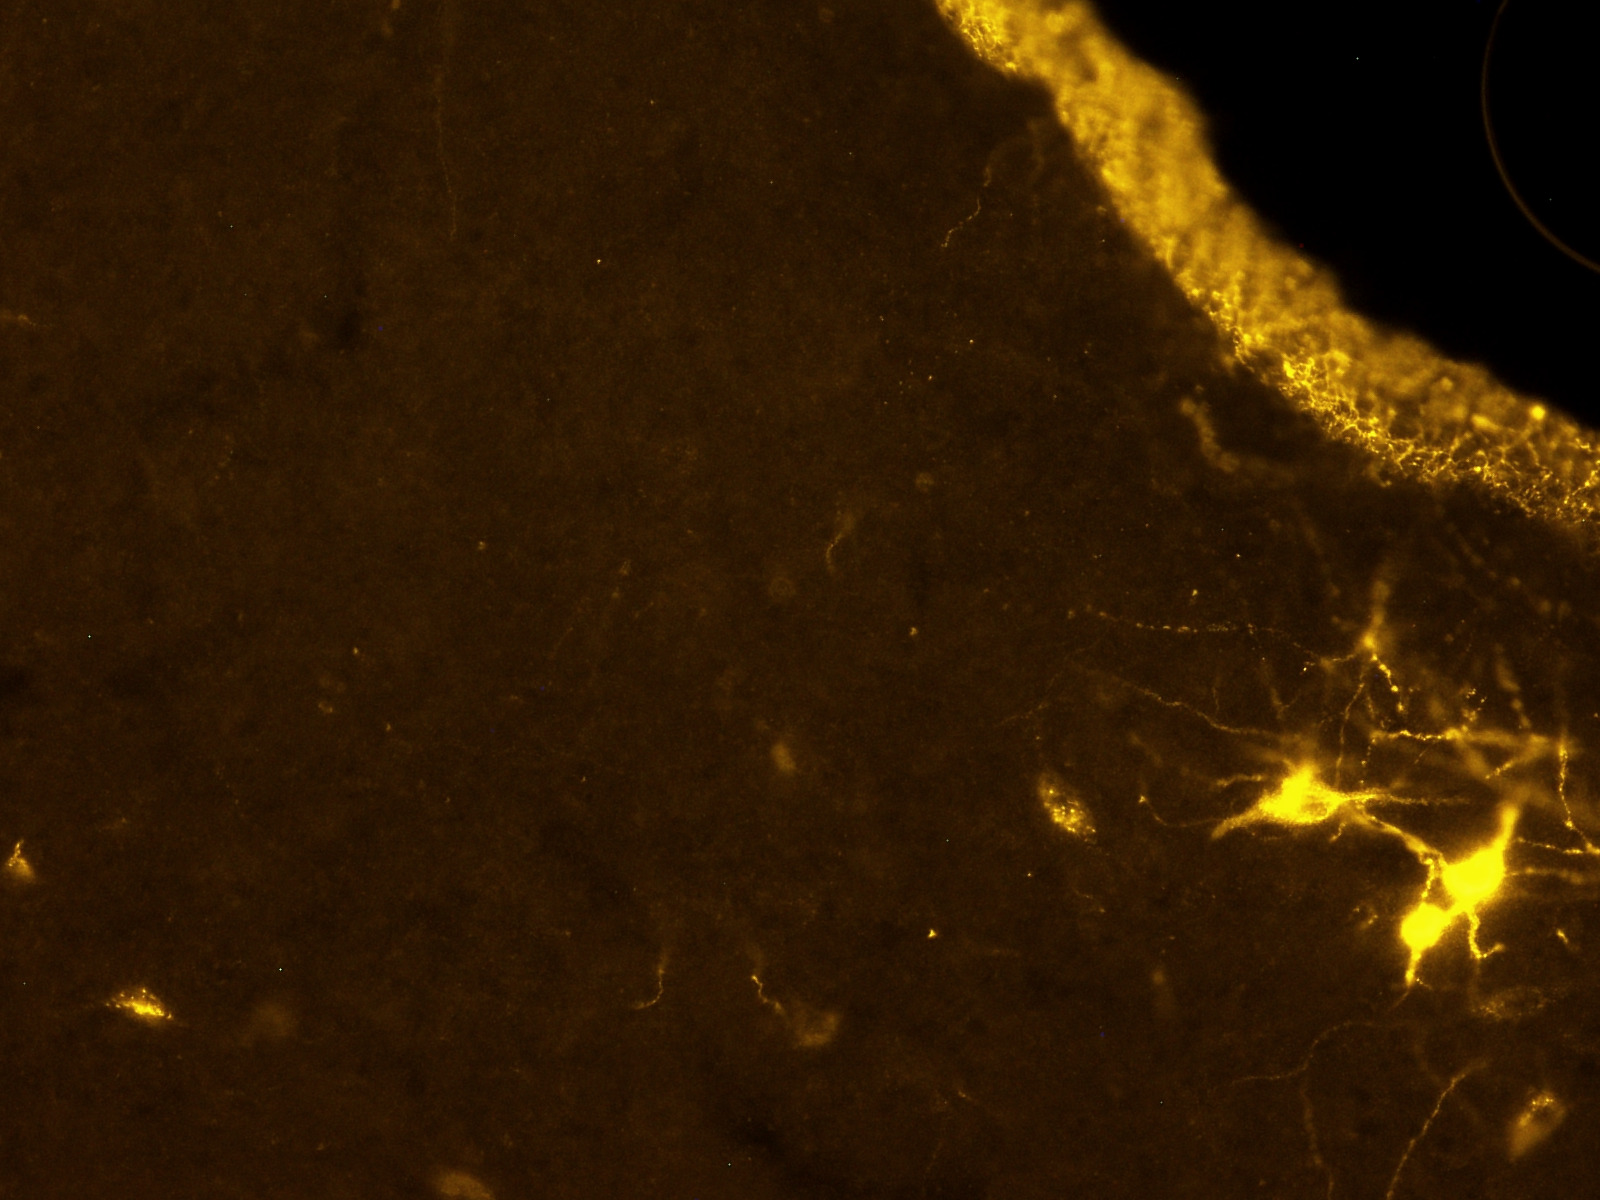
\includegraphics[width=0.55\textwidth]{figures/120_dataset/i_252.jpeg}
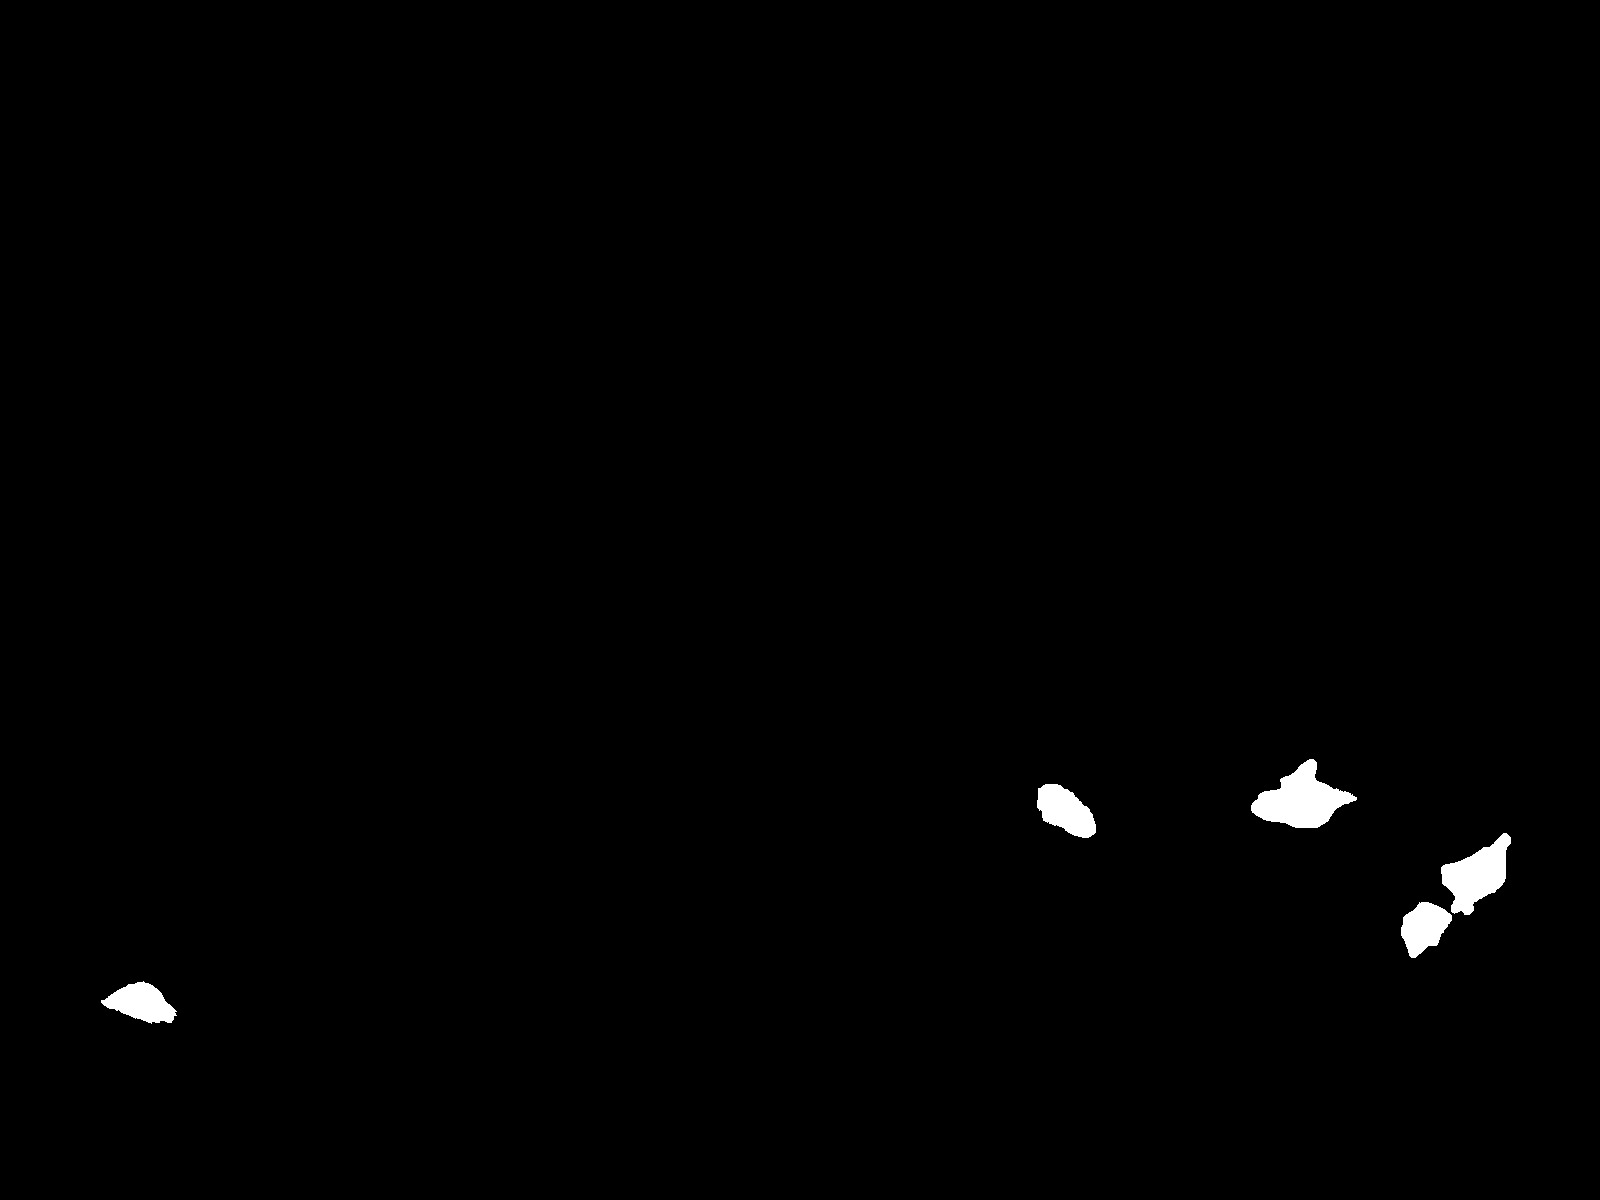
\includegraphics[width=0.55\textwidth]{figures/120_dataset/m_252.jpeg}
}
\centerline{
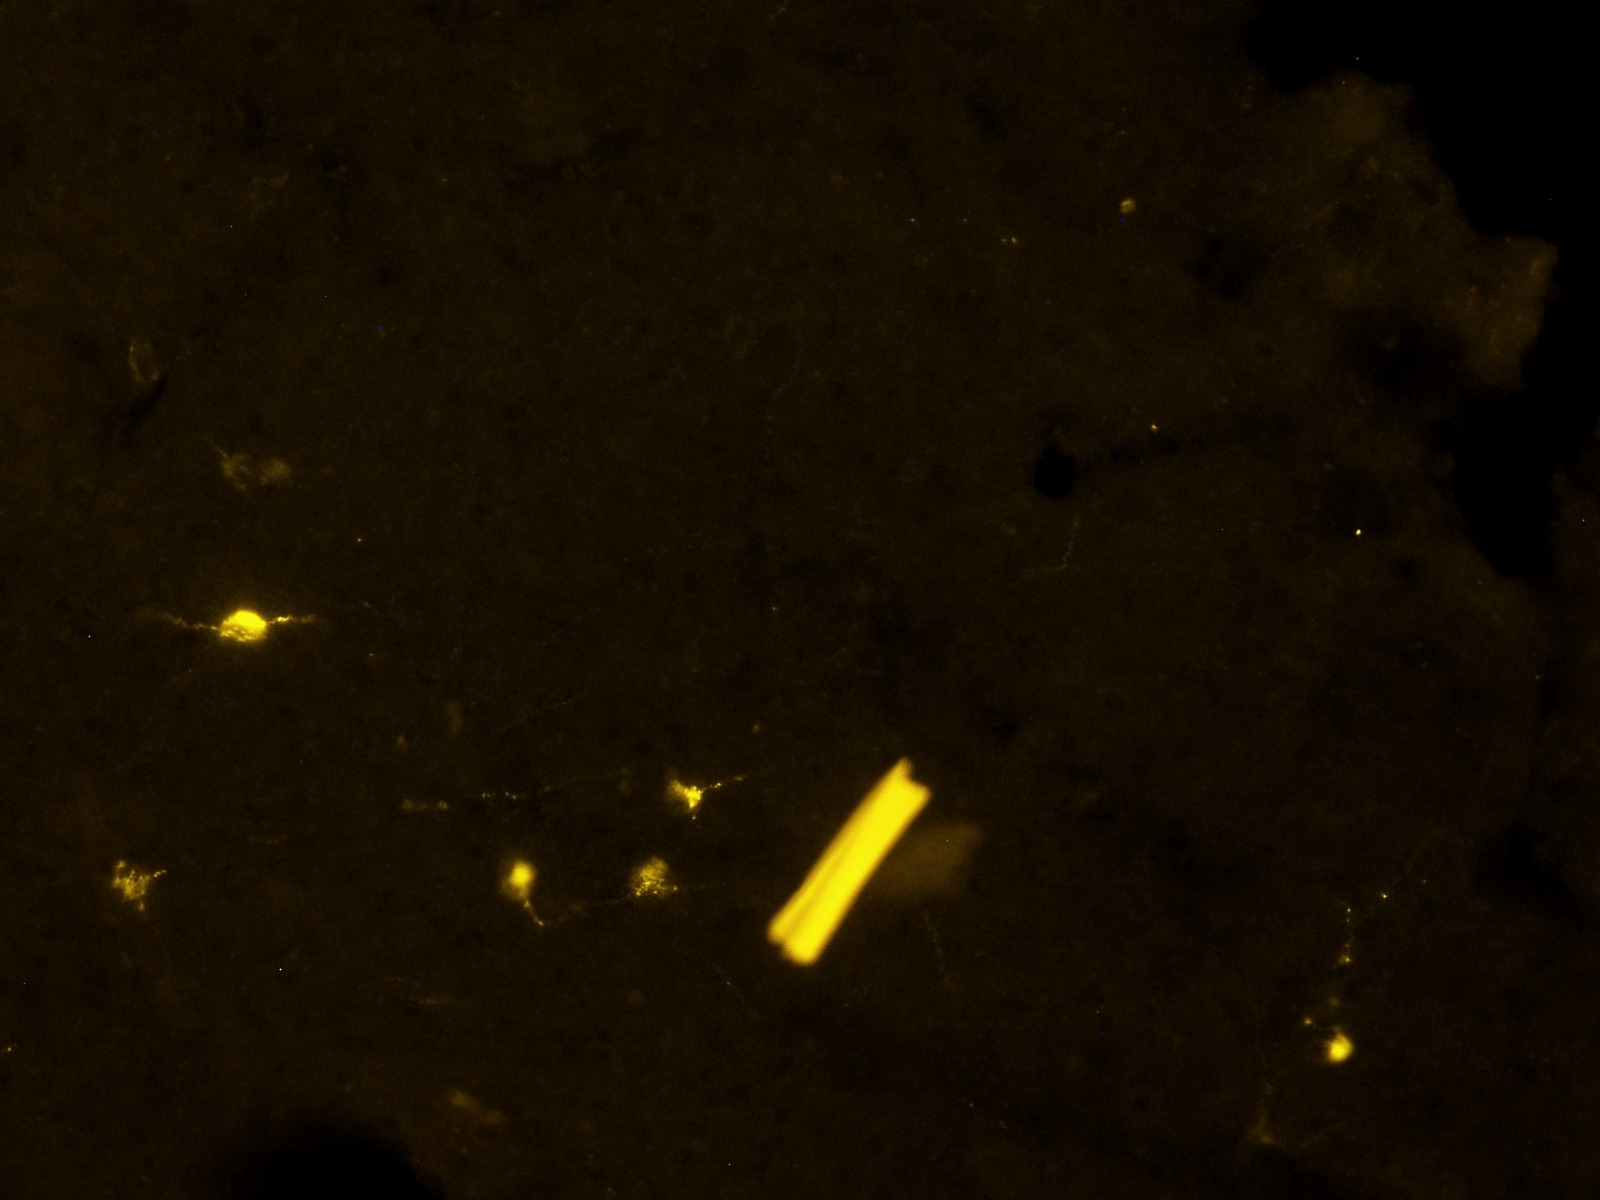
\includegraphics[width=0.55\textwidth]{figures/120_dataset/i_maccherone.jpeg}
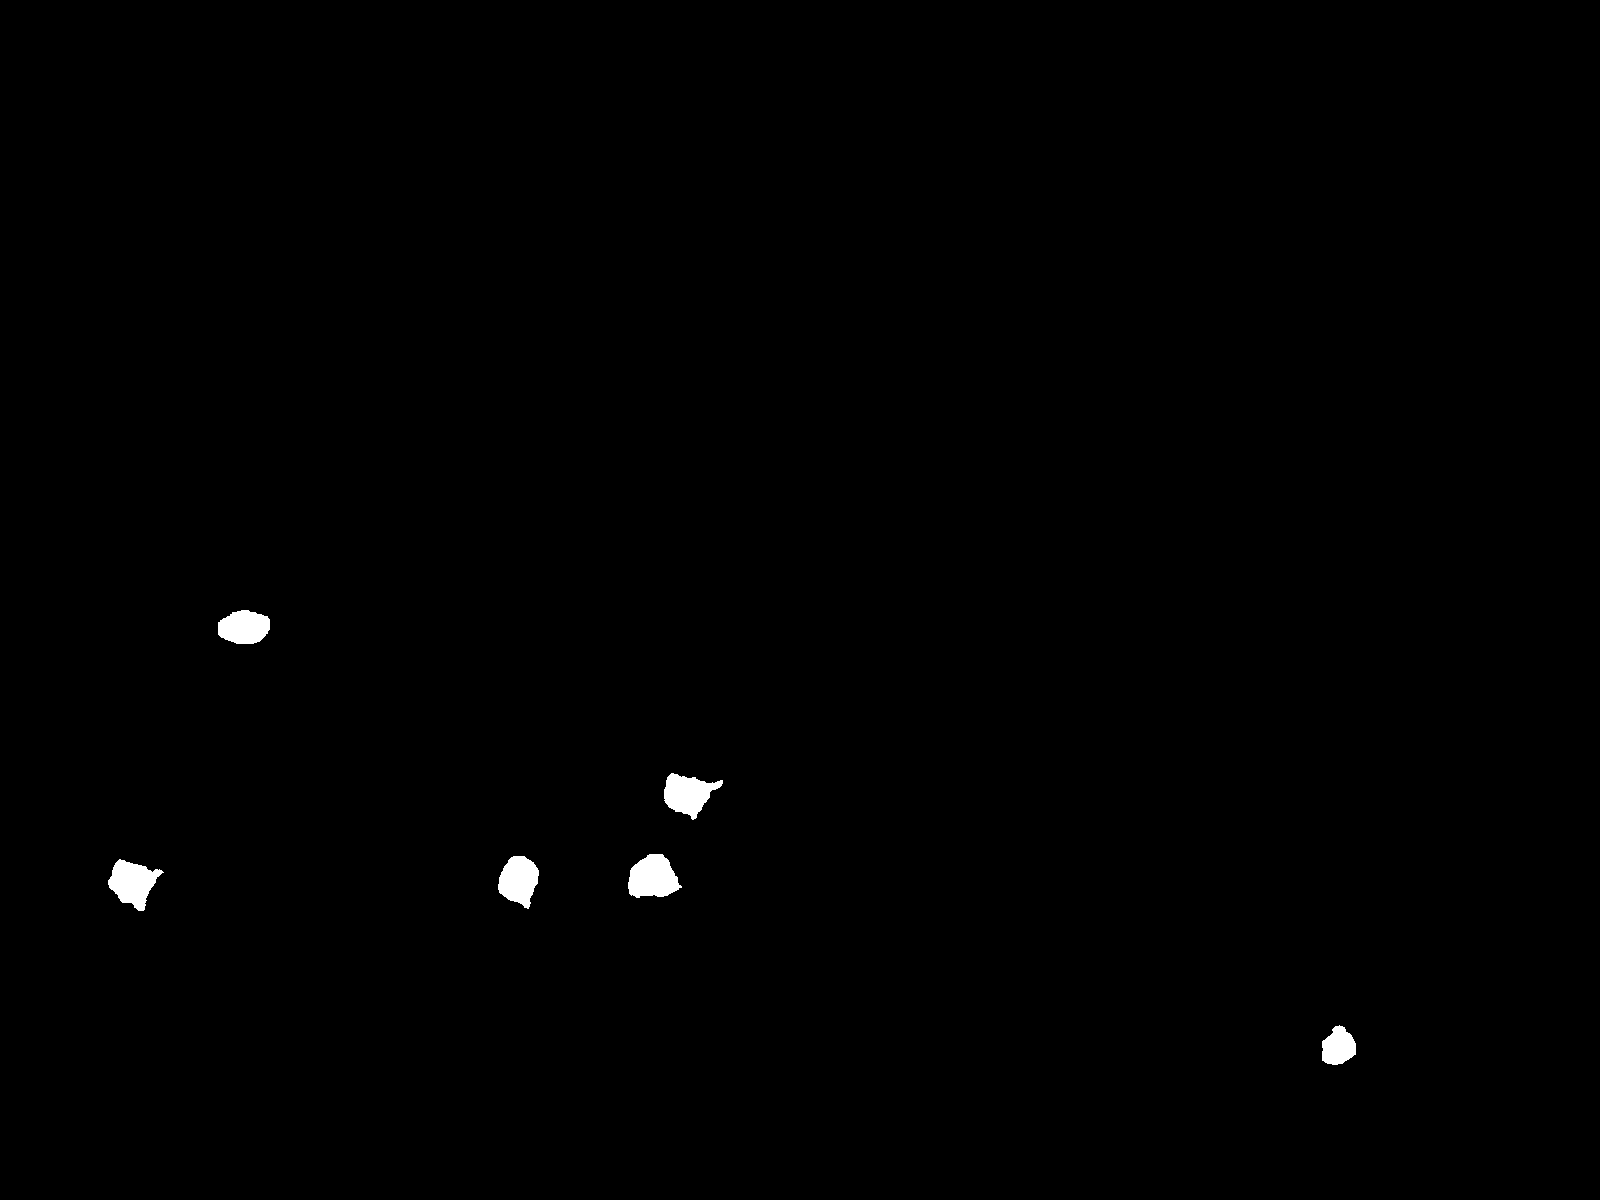
\includegraphics[width=0.55\textwidth]{figures/120_dataset/m_maccherone.png}
}
\caption{
\textbf{Sample data}. The original images (left) present neuronal cells of different shape, size and saturation over a background of variable brightness and color.
The corresponding ground-truth masks used for training (right) depicts cells as white pixels over a black background.
%%rephrase
% \textbf{Sample data}. In the original images (left), the neuronal cells of interest appear as yellow spots over a background of variable brightness and color. They exhibit a large variability in terms of shape, size and saturation, which makes them hard to distinguish from artifacts and similar biological structures that are not of interest.
% The corresponding ground-truth masks used for training (right) depicts cells as white pixels over a black background.
} 
\label{fig:dataset}
\end{figure}

The \textbf{Fluorescent Neuronal Cells} dataset \cite{clissa2021fluocells} consists of 283 high-resolution pictures (1600$\times$1200 pixels) of mice brain slices and the corresponding ground-truth labels.
The mice were subjected to controlled experimental conditions, and a monosynaptic retrograde tracer (Cholera Toxin b, CTb) was surgically injected into brain tissues to highlight the neurons connected to the injection site
%projecting to the injection site
\cite{hitrec2019neural}.
Specimens of brain slices were then observed through  
a fluorescence microscope configured to select the narrow wavelength of light emitted by 
a fluorophore (of a yellow/orange color) associated with the tracer.
Thus, the resultant images depict neurons of interest as objects of different size and shape appearing as yellow-ish spots of variable brightness and saturation over a composite, generally darker background (Fig. \ref{fig:dataset}, left).

Although many efforts were made to stabilize the acquisition procedure, the images present several relevant challenges for the detection task. 
In fact, the variability in brightness and contrast causes some fickleness in the pictures overall appearance.  
Also, the cells themselves exhibit varying saturation levels due to the natural fluctuation of the fluorescent emission properties. 
Moreover, the substructures of interest have a fluid nature. This implies that the shape of the stained cells may change significantly, making it even harder to discriminate between them and the background. 
Combined to that, artifacts, bright biological structures -- like neurons' filaments -- and non-marked cells similar to the stained ones handicap the recognition task. 
Besides complicating the training, all of these factors %make the goal of this work more challenging and
likewise hinder model evaluation as the interpretation of such borderline cases becomes subjective.

Finally, another source of complexity is the broad shift in the number of target cells from image to image.
Indeed, the total counts range from no stained cells to several dozens clumping together. 
In the former case, the model needs high precision in order to prevent false positives. The latter, instead,
requires high recall since considering two or more touching neurons only once produces false negatives. 

\section{Ground-truth labels}
Under a supervised learning framework, the training phase leverages ground-truth labels acting as examples of desired outputs that the model should learn to reproduce. In the case of image segmentation, such targets are in the form of binary images (\textit{masks}) where the objects to segment and the background are represented by white and black pixels, respectively (Fig. \ref{fig:dataset}, bottom row).

Obtaining target masks usually requires a great effort in terms of time and human resources, so we resorted to an automatic procedure to speed up the labeling. 
In particular, we started from a large subset composed by 252 images and applied gaussian blurring to remove noise. The cleaned images were then subjected to a thresholding operation based on automatic histogram shape-based methods. 
The goal was to obtain a loose selection of the objects that may seem good candidates to be labeled as neuronal cells. 
After that, acknowledged operators reviewed the results to discard the false positives introduced with the previous procedure, taking care of excluding irrelevant artifacts and misleading biological structures.
The remaining images were segmented manually by domain experts. We included significant pictures with peculiar traits -- such as artifacts, filaments and crowded objects -- in the latter set to have highly reliable masks for the most challenging examples 
% (see $link_to_github$ for more details)
.

% \lc{A summary of the distributions of counts and objects features is presented in Table \ref{tab:dataset_summary}}.
% % ...possibly add geometrical information of cell objects, average/median/max/min counts per image, ... others(?)
% \begin{table}[b]
% \begin{center}
% \begin{tabular}{cccccc}
% \hline
% area    & minor axis & major axis & equivalent diameter & maximum feret diameter & mean diameter \\
% \hline
% 1206.43 & 29.39 & 50.43 & 36.50 & 55.34 & 47.42\\
% \hline
% \end{tabular}
% \caption{Summary statistics of cells morphological features (measured in pixels)}
% \label{tab:dataset_summary}
% \end{center}
% \end{table}


Despite the huge popularity Deep Learning has gained in computer vision in the last decade, the lack of annotated data is a common curse when dealing with applications involving non-standard pictures and/or tasks \cite{curse_dataset_annotation}. 
Since ground-truth labels are expensive to acquire in terms of time and costs, a common approach is to fine-tune models pre-trained on giants datasets of natural images like ImageNet \cite{ImageNet} or COCO \cite{COCO}, possibly using as few new labels as possible for the task of interest. 
However, this strategy often does not apply to use cases where the pictures under analysis belong to extraneous domains with respect to the ones used for pre-training \cite{TL_medical_imaging}.
For this reason, by releasing the annotated dataset and our pre-trained model we hope to \textit{i)} foster advances in fields like biomedical imaging through the speed up guaranteed by the automation of manual operations, and \textit{ii)} promote methodological research on new techniques of data analysis for microscopic fluorescence and similar domains.